\documentclass{ctexart}
\usepackage[a4paper,total={6in,8in}]{geometry}
\usepackage{fancyhdr}
\usepackage[table,xcdraw]{xcolor}
\usepackage[utf8]{inputenc}
\usepackage{ctex}
\usepackage{color}
\usepackage{subfigure}
\usepackage{cite}
\usepackage{graphicx}
\usepackage{fontspec}
\setmainfont{Times New Roman}
\newfontfamily\timesfont{Times New Roman}
\usepackage{CJK}
\usepackage{indentfirst}
\usepackage{amsmath}
\usepackage{mathrsfs}
\usepackage{multirow}
\usepackage{svg}
\usepackage{amsfonts}
\usepackage{geometry}
\usepackage{hyperref}
\usepackage{mathabx}
\usepackage{cases}
\usepackage{minipage-marginpar}
\usepackage{xcolor}
% 导入包
\usepackage{hyperref}
% 格式设置
\hypersetup{hidelinks,
	colorlinks=true,
	allcolors=blue,
	pdfstartview=Fit,
	breaklinks=true}

\begin{document}

\begin{titlepage}
    \title{{\fontsize{28}{32}\selectfont\kaishu 机器人学 \\ \fontsize{20}{24}\selectfont\kaishu{作业5:运动学轨迹规划}}}
    \date{} % delete date as you want
    \maketitle
    \vspace{-7em}
    \begin{center}
      \fontsize{18}{22}\selectfont
      \textbf{\timesfont Robotics (2023-2024-2) \\
      Homework 5: Kinematic Trajectory Planning}
    \end{center}
    
    \begin{figure}[h]
        \centering
        
\includegraphics[width=0.45\textwidth]{Image/校标-校徽.png}
    \end{figure}
    \begin{center}
      \hspace{6em}
      \renewcommand{\arraystretch}{2}
      \begin{tabular}{rl}
      \fontsize{16}{50}\selectfont\heiti 姓名:& \fontsize{16}{24}\selectfont\heiti 赵四维 \\
      \fontsize{16}{24}\selectfont\heiti 学号:& \fontsize{16}{24}\selectfont 521021910696 \\
      \fontsize{16}{24}\selectfont\heiti 班级:& \fontsize{16}{24}\selectfont ME3403-01 \\
      \fontsize{16}{24}\selectfont\timesfont E-mail:& \fontsize{16}{24}\selectfont racheus.11@sjtu.edu.cn \\
      \end{tabular}
    \end{center}
    \begin{center}
      \fontsize{16}{24}\selectfont\timesfont \today
    \end{center}
\end{titlepage}

\pagenumbering{arabic}

\newpage
% \tableofcontents


\newpage
\pagestyle{fancy}
\fancyhf{}
\fancyhead[L]{ME3403-01}
\fancyhead[C]{机器人学Homework2}
\fancyhead[R]{赵四维 521021910696}
\fancyfoot[C]{\thepage}
\section*{旋转矩阵的求取、变换和证明}
\subsection*{1.求旋转矩阵它表示坐标系\{B\}(一开始与\{A\}重合)经过了如下运动:(a) 绕$x_B$旋转$60^\circ$;(b) 绕$z_B$旋转$60^\circ$; (c) 绕$z_A$旋转$90^\circ$。}
[Solution]:\par

\href{src/Rhw_2_1_main.m}{Click here to jump to the MATLAB code.}\par

先给出(a)、(b)、(c)三个旋转矩阵的表达式:
\begin{equation}
	R_{x_B}(\theta) = \begin{bmatrix}
		1 & 0 & 0 \\
		0 & \cos\theta & -\sin\theta \\
		0 & \sin\theta & \cos\theta
	\end{bmatrix}=
	\begin{bmatrix}
		1 & 0 & 0 \\
		0 & \frac{1}{2} & -\frac{\sqrt{3}}{2} \\
		0 & \frac{\sqrt{3}}{2} & \frac{1}{2}
	\end{bmatrix}
\end{equation}
\begin{equation}
	R_{z_B}(\theta) = \begin{bmatrix}
		\cos\theta & -\sin\theta & 0 \\
		\sin\theta & \cos\theta & 0 \\
		0 & 0 & 1
	\end{bmatrix}=
	\begin{bmatrix}
		\frac{1}{2} & -\frac{\sqrt{3}}{2} & 0 \\
		\frac{\sqrt{3}}{2} & \frac{1}{2} & 0 \\
		0 & 0 & 1
	\end{bmatrix}
\end{equation}
\begin{equation}
	R_{z_A}(\theta) = \begin{bmatrix}
		\cos\theta & -\sin\theta & 0 \\
		\sin\theta & \cos\theta & 0 \\
		0 & 0 & 1
	\end{bmatrix}=
	\begin{bmatrix}
		0 & -1 & 0 \\
		1 & 0 & 0 \\
		0 & 0 & 1
	\end{bmatrix}
\end{equation}

注意到(1)、(2)两个变换是在\{B\}坐标系下进行的,是"Euler Angle"范畴,在求矩阵的过程中要\textbf{右乘};而(3)是在\{A\}坐标系下进行的,是"Fixed Angle"范畴,在求矩阵的过程中要\textbf{左乘}。

因此,最终旋转矩阵为:

\begin{equation*}
	R = R_{z_A}(\theta)R_{x_B}(\theta)R_{z_B}(\theta) = \begin{bmatrix}
		0 & -1 & 0 \\
		1 & 0 & 0 \\
		0 & 0 & 1
	\end{bmatrix}\begin{bmatrix}
		1 & 0 & 0 \\
		0 & \frac{1}{2} & -\frac{\sqrt{3}}{2} \\
		0 & \frac{\sqrt{3}}{2} & \frac{1}{2}
	\end{bmatrix}\begin{bmatrix}
		\frac{1}{2} & -\frac{\sqrt{3}}{2} & 0 \\
		\frac{\sqrt{3}}{2} & \frac{1}{2} & 0 \\
		0 & 0 & 1
	\end{bmatrix}=
	\begin{bmatrix}
		-0.433 & -0.25 & 0.866 \\
		0.50 & -0.866 & 0 \\
		0.75 & 0.433 & 0.5\\
	\end{bmatrix}
\end{equation*}

\subsection*{2.已知坐标系\{B\}相对于坐标系\{A\}的齐次变换矩阵为}

$$
\begin{bmatrix}
	? & 0 & 1 & 1 \\
	? & 0 & 0 & 2 \\
	? & -1 & 0 & 3 \\
	? & 0 & 0 & 1
\end{bmatrix}
$$
\textbf{(1)求第一列元素的值\\(2)求旋转运动的旋转轴和旋转角\\(3)若$p^A=[1,3,5]^T$,求$p^B$} 

[Solution]:\par

(1)由增广后旋转矩阵的定义,$R_{41}=0$是显然的。而矩阵的前三行前三列(记为$R^\prime = [q_1,q_2,q_3]$)构成的$3\times 3$矩阵是一个\textbf{正交矩阵},且行列式为1。因此,设$R_{11}=a,R_{21}=b,R_{31}=c$,则有:
\begin{equation}
	\begin{cases}
		q_1 \cdot q_2 = 0 \rightarrow c = 0\\
		q_1 \cdot q_3 = 0 \rightarrow a = 0\\
		det(R^\prime) = 1 \rightarrow (-1)^{(1+3)}b\times(-1)=1 \rightarrow b = -1\\
	\end{cases}
\end{equation}

因此,旋转矩阵的表示为:

\begin{equation}
	R = \begin{bmatrix}
		0 & 0 & 1 & 1 \\
		-1 & 0 & 0 & 2 \\
		0 & -1 & 0 & 3 \\
		0 & 0 & 0 & 1
	\end{bmatrix}
\end{equation}

(2) \href{src/Rhw_2_2_main.m}{Click here to jump to the MATLAB code.}\par

本小题采用MATLAB的\verb|rotm2axang|函数,该函数可以将旋转矩阵转换为旋转轴和旋转角。

\begin{figure}[h]
	\centering
	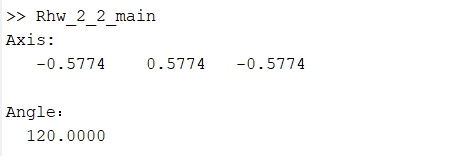
\includegraphics[width=0.8\textwidth]{Image/2_2.png}
	\caption{旋转矩阵转换为旋转轴和旋转角}
\end{figure}

因此旋转轴为$\mathbf{e} =[-0.5774,0.5774,-0.5774]$,旋转角为$\psi =120^\circ$。

(3)由题意,$p^A=[1,3,5]^T$,增广为$[1,3,5,1]^T$。则有:

\begin{equation}
	p^B = \begin{bmatrix}
		0 & 0 & 1 & 1 \\
		-1 & 0 & 0 & 2 \\
		0 & -1 & 0 & 3 \\
		0 & 0 & 0 & 1
	\end{bmatrix}\begin{bmatrix}
		1 \\
		3 \\
		5 \\
		1
	\end{bmatrix} = \begin{bmatrix}
		6 \\
		1 \\
		0 \\
		1
	\end{bmatrix}
\end{equation}

因此,$p^B = [6,1,0]^T$。

\subsection*{3.设R是一个旋转矩阵,求证$\det{R}=1$(坐标系为右手系)}

[Proof:]\par

由于旋转矩阵是一个\textbf{正交矩阵},由正交矩阵的性质$R^TR=I$。因此有:

\begin{equation}
	|R^TR| = |I| = 1
\end{equation}

由行列式的性质$|AB| = |A||B|$,又由矩阵转置的性质$|A|=|A^T|$,因此有:

\begin{equation}
	|R^TR| = |R^T||R| = |R||R| = (\det{R})^2 = 1
\end{equation}

因此有$|R| = \pm 1$。由题意,在右手系下参考,正交矩阵的n个列向量组成的标准正交基,行列式必定为\textbf{正数}。因此有$\det{R}=1$,证毕。

\section*{MATLAB编程题}

\subsection*{4.MATLAB 函数“eul2rotm”可以将欧拉角向量转化为旋转矩阵,而“rotm2eul”函数可以实现旋转矩阵到欧拉角的反解。该函数有一个选项可决定旋转轴顺序,选择“ZYX”顺序。已知测试数据如表 1 所示,完成以下任务:}
\begin{table}[h]
	\centering
	\begin{tabular}{ccc}
	\hline
	$\alpha$ & $\beta$ & $\gamma$ \\ \hline
	10       & 20      & 30       \\ 
	30       & 90      & -55      \\ \hline
	\end{tabular}
	\end{table}
\textbf{1)	使用第一行数据和“rotx”“roty”“rotz”函数验证“eul2rotm”是绕定轴旋转的还是绕动轴旋转的,并给出eul2rotm($\mathbf{[\alpha,\beta,\gamma],'ZYX'}$)对应的绕 xyz 轴分解式。}

\textbf{2)	实现该顺序的旋转矩阵-欧拉角反解程序,并将反解结果与 “rotm2eul”函数的反解结果、原参数作对比。请问结果与原参数是否相 同?若不相同,请解释原因。
}

[Solution]:\par

(1) \href{src/Rhw_2_4_main.m}{Click here to jump to the MATLAB code.}\par

由MATLAB计算得到的结果,可见结果是绕\textbf{动轴}旋转的,即以每次旋转变换后的坐标系作为新的参考系进行旋转,在矩阵乘法的过程中体现为\textbf{右乘}。

同样,由MATLAB计算得到的结果,如果绕‘XYZ’顺序旋转,那么得到的分解式(Euler Angle)为:$[10^\circ,20^\circ,30^\circ]$。

(2) \href{src/Rhw_2_4_2_main.m}{Click here to jump to the MATLAB code.}\par

由MATLAB计算得到的结果,可以看到,旋转矩阵-欧拉角反解程序的结果与“rotm2eul”函数的反解结果、原参数是\textbf{相同}的。

因为在本题的求解过程中笔者使用了\verb|atan2|函数,这一函数已在第一次作业中有所说明。该函数在机器人学中至关重要,其优势在于可以正确地处理四个象限的所有角度,并且避免了由于负数或者除数为0时而产生的错误。因此,可以保证结果的正确性。

$$\arctan2(y,x) = \begin{cases}
	\arctan(\frac{y}{x}) & x>0 \\
	\arctan(\frac{y}{x})+\pi & x<0,y\geq 0 \\
	\arctan(\frac{y}{x})-\pi & x<0,y<0 \\
	\frac{\pi}{2} & x=0,y>0 \\
	-\frac{\pi}{2} & x=0,y<0 \\
	\text{undefined} & x=0,y=0		
\end{cases}$$															

\subsection*{5.实现齐次变换矩阵求逆函数,并与 MATLAB 函数 inv 比较运算结果 和运算时间。}

\href{src/Rhw_2_5_main.m}{Click here to jump to the MATLAB code.}\par

基本解决思路为:
$$
T^B_A = \begin{bmatrix}
	R^B_A & p^B_{A0} \\
	0 & 1
\end{bmatrix}
= \begin{bmatrix}
	(R_B^A)^T & -R_B^Ap^B_{A0} \\
	0 & 1
\end{bmatrix}
=(T_B^A)^{-1}
$$

在MATLAB中分别用自己的求逆函数和自带的inv函数,得到的结果是相同的。分别循环$10^4$次,求逆函数的运算时间为$0.0370s$,而inv函数的运算时间为$0.0060s$。因此,可以MATLAB自带的inv函数的运算速度更快。

\begin{figure}[h]
	\centering
	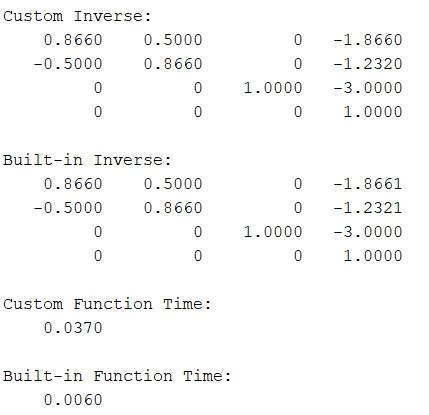
\includegraphics[width=0.45\textwidth]{Image/2-5.png}
	\caption{齐次变换矩阵求逆函数与MATLAB函数inv函数求解时间对比}
\end{figure}


\textbf{代码块 { }  { } 求逆函数}\par

\vspace{5pt}
\hrule

\begin{verbatim}
	function T_inv = inverse_homogeneous_transform(T)
    R = T(1:3, 1:3);
    p = T(1:3, 4);
 
    % Rotation matrix inv
    R_inv = R';
    
    % inverse of translation part
    p_inv = -R_inv * p;
    
    % Remake a new homogeneous transformation matrix
    T_inv = eye(4);
    T_inv(1:3, 1:3) = R_inv;
    T_inv(1:3, 4) = p_inv;
end
\end{verbatim}
\hrule
\vspace{5pt}

分析其原因,经过观察,在我自己的求逆函数中,有两次矩阵提取运算,有一次转置运算,一次\textbf{矩阵乘法},七次赋值运算,其中除了矩阵乘法的复杂度是O($n^2$)外,其他的复杂度都是O($n$)。在矩阵规模较小的时候,时间差异不明显,因此笔者采用循环$10^4$次的方式来进行对比。

经查阅资料,MATLAB内置函数使用了一些高效的数值计算算法,这些算法经过了精心设计和优化,以在各种情况下都能提供良好的性能。包括但不限于LU分解、QR分解、特征值分解等方法,可以使得inv函数的运算速度更快$^{[1]}$。

*同样,笔者已将代码上传至\href{https://github.com/Racheus/Robotics-Caprice/tree/master/Homework2-Mathematic-foundations}{here}。若文中链接有无法打开的情况,烦请助教老师点击查看。
\section*{Reference}

[1]MATLAB Documentation. (n.d.). Retrieved October 10, 2021, from \url{https://ww2.mathworks.cn/help/matlab/}


\end{document}

